%!TEX TS-program = xelatex
%!TEX encoding = UTF-8 Unicode

% Modify the following line to match your school
% Available options include `Harvard`, `Princeton`, and `NYU`.
\documentclass[School=Harvard]{Dissertate}

\usepackage{color}
\definecolor{bluekeywords}{rgb}{0.13,0.13,1}
\definecolor{greencomments}{rgb}{0,0.5,0}
\definecolor{redstrings}{rgb}{0.9,0,0}
\definecolor{grey}{rgb}{0.5,0.5,0.5}

\usepackage{listings}
\lstset{language=Python,
basicstyle=\footnotesize\ttfamily,
breakatwhitespace=false,
breaklines=false,
commentstyle=\color{greencomments},
escapeinside={(*@}{@*)},
keywordstyle=\color{bluekeywords}\bfseries,
numbers=left,
numbersep=5pt,
numberstyle=\tiny\color{grey},
showspaces=false,
showstringspaces=false,
showtabs=false,
stringstyle=\color{redstrings}
}

%\lstset{
%    basicstyle=\footnotesize\ttfamily,
%    breaklines=false,
%    language=Python,
%    showspaces=false, 
%    showstringspaces=false
%}

\begin{document}

% the front matter
% Some details about the dissertation.
\title{How to cook an egg}
\author{Josiah Wolf Oberholtzer}
\advisor{Hans Tutschku \& Chaya Czernowin}

% ... about the degree.
\degree{Doctor of Philosophy}
\field{Music Composition}
\degreeyear{2015}
\degreemonth{May}
\department{Music}

% ... about the candidate's previous degrees.
\pdOneName{B.Mus.}
\pdOneSchool{Oberlin Conservatory}
\pdOneYear{2006}

%\pdTwoName{M.A.}
%\pdTwoSchool{Monster's Univeristy}
%\pdTwoYear{2021}
\maketitle
\copyrightpage
\abstractpage
\tableofcontents
%\authorlist
\listoffigures
\dedicationpage
\acknowledgments

\doublespacing

% include each chapter...
\setcounter{chapter}{-1}  % start chapter numbering at 0
%%%%%%%%%%%%%%%%%%%%%%%%%%%%%%%%%%%%%%%%%%%%%%%%%%%%%%%%%%%%%%%%%%%%%%%%%%%%%%%%
%%%%%%%%%%%%%%%%%%%%%%%%%%%%%%%%%%%%%%%%%%%%%%%%%%%%%%%%%%%%%%%%%%%%%%%%%%%%%%%
\chapter{Introduction}
\label{chap:introduction}
%%%%%%%%%%%%%%%%%%%%%%%%%%%%%%%%%%%%%%%%%%%%%%%%%%%%%%%%%%%%%%%%%%%%%%%%%%%%%%%
%%%%%%%%%%%%%%%%%%%%%%%%%%%%%%%%%%%%%%%%%%%%%%%%%%%%%%%%%%%%%%%%%%%%%%%%%%%%%%%

\begin{figure}
\begin{centering}
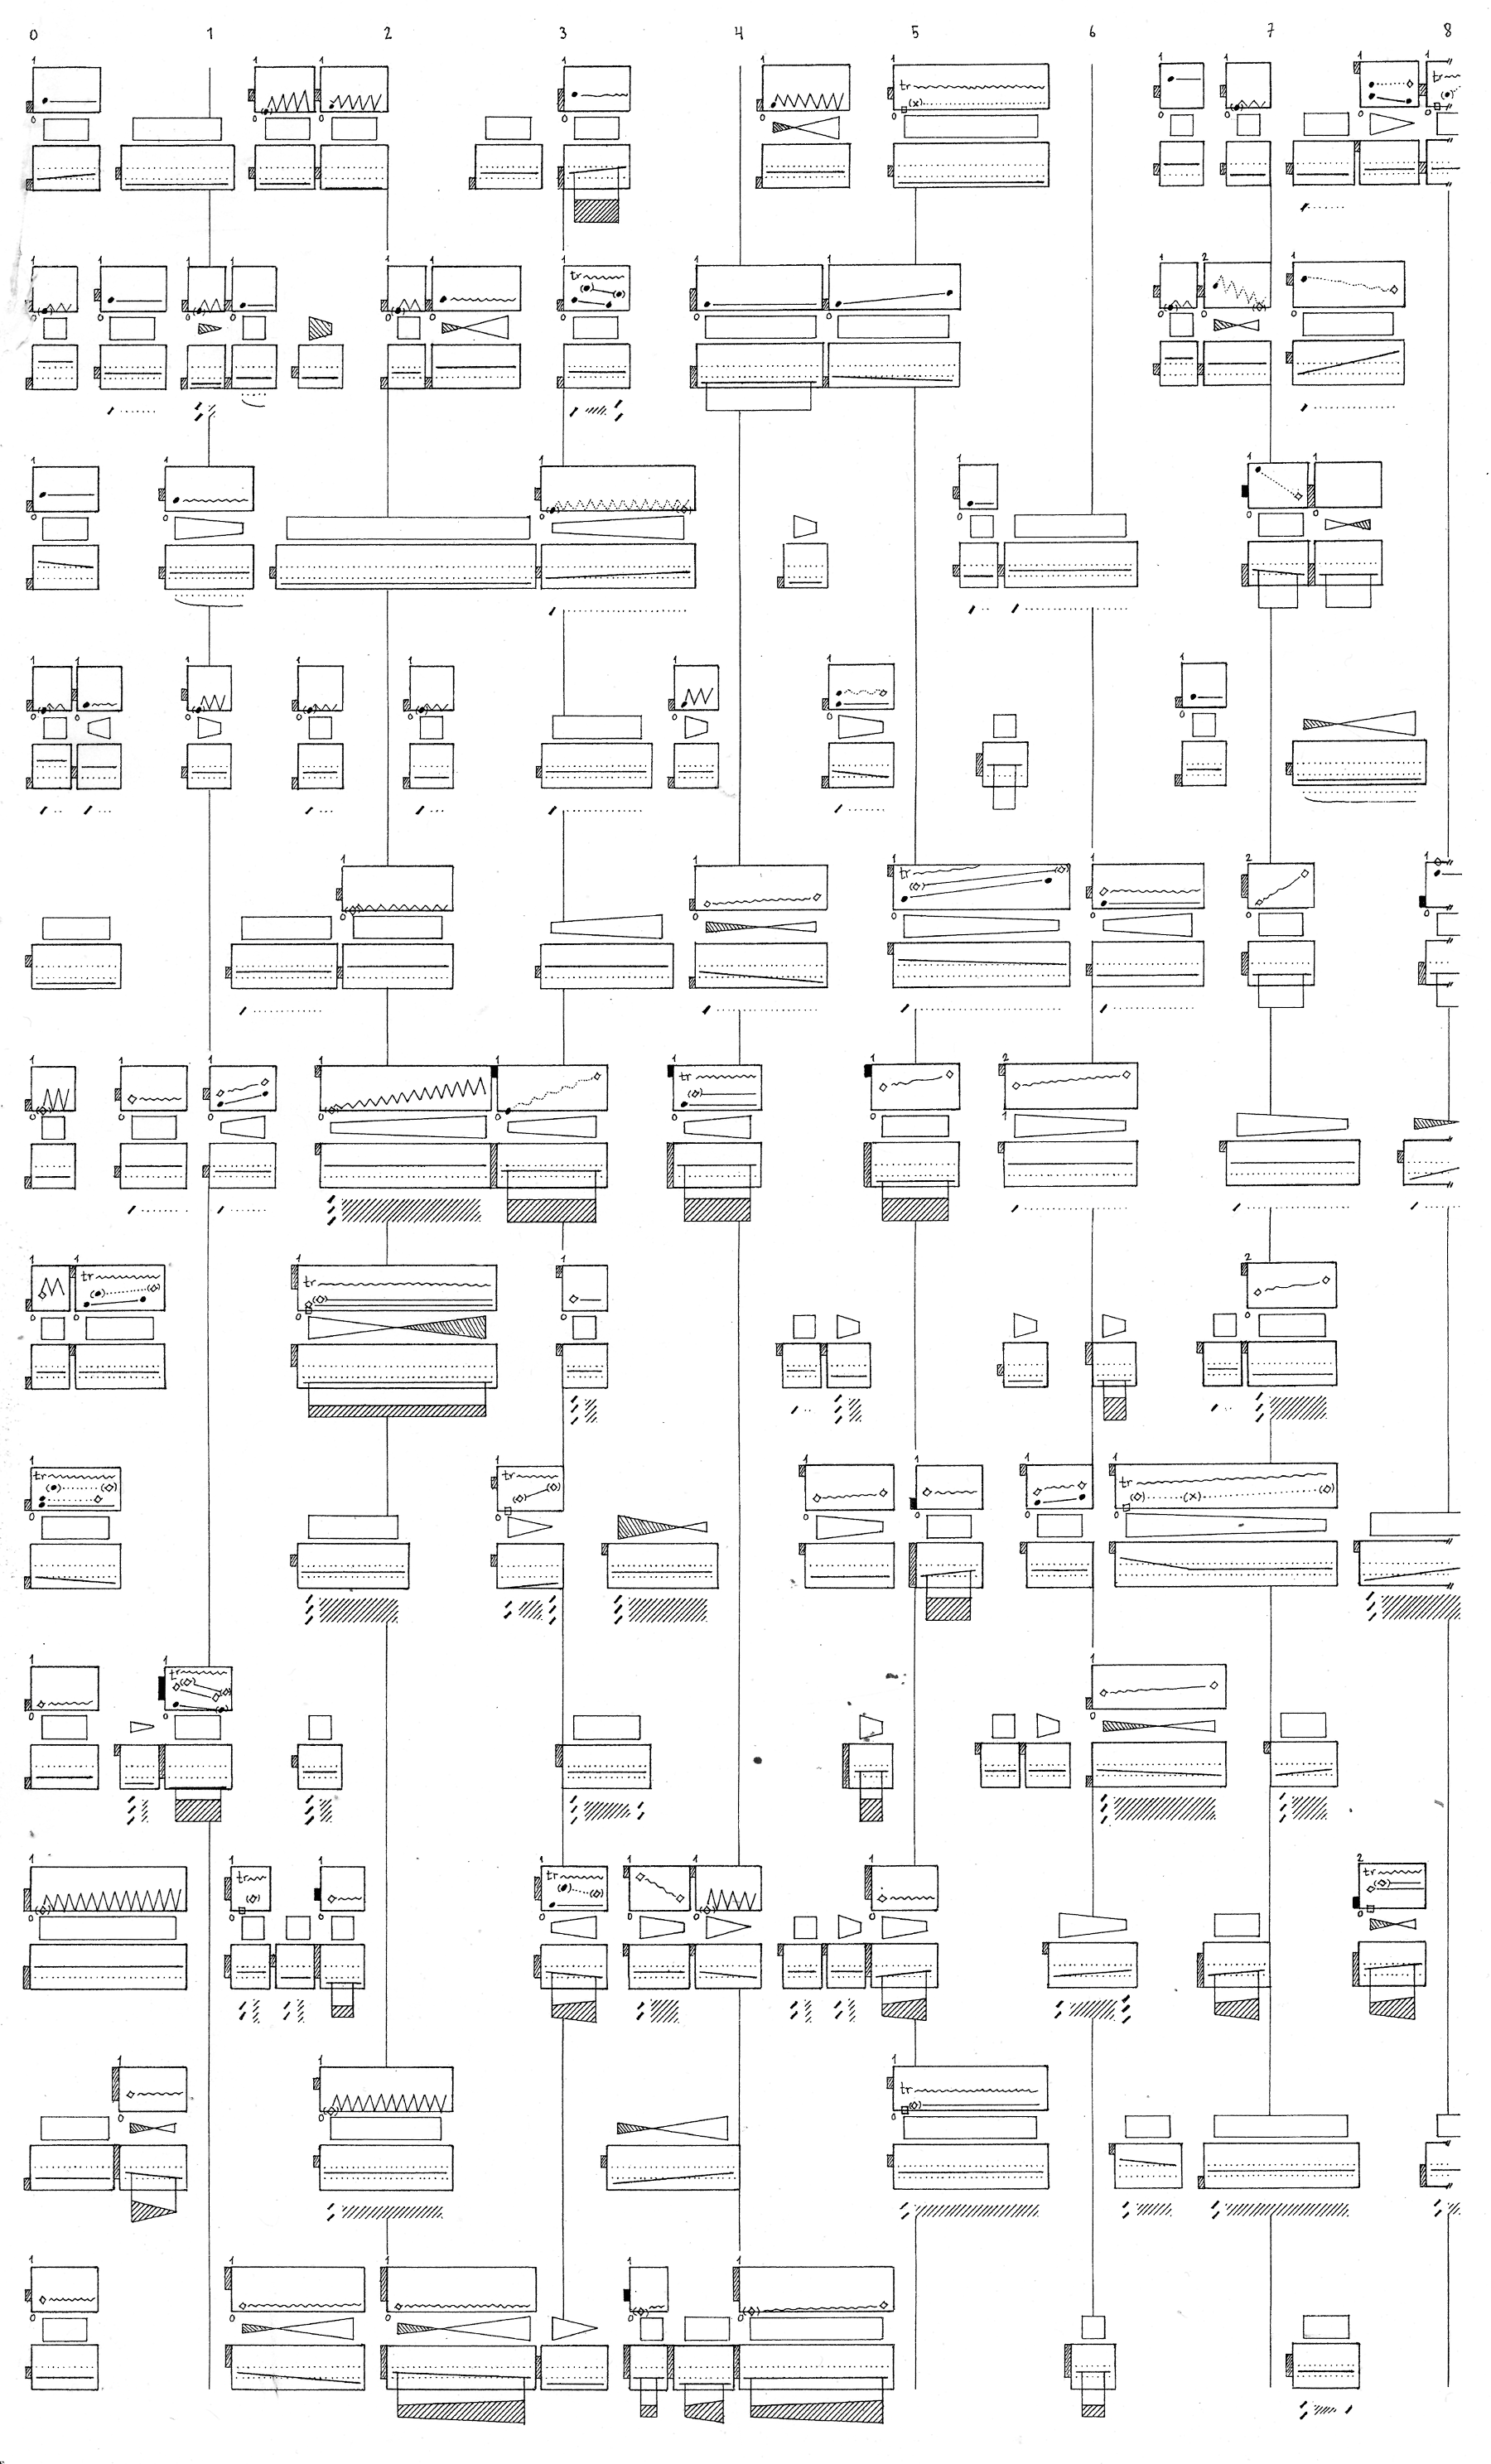
\includegraphics[
    page=1,
    width=\textwidth,
    height=0.9\textheight,
    keepaspectratio,
]{assets/dissertation-score-mbrsi.pdf}
\caption{The first page of \emph{mbrsi} (2006), an unfinished tablature score
for one to twelve string performers. This represents an early attempt of mine
at computationally modeling massed performers with timespans to create an
evolving \enquote{granular} texture. The instructions for the score were
created through a variety of Max/MSP patches which painstakingly converted
noise functions into text files which I then collated into spreadsheets. The
score itself was drawn by hand on size A1 graph paper with Rapidographs.
I completed seventeen of the intended fifty-three pages before stopping for the
sake of my wrists and due a general lack of faith in the project. While still
incomplete, the concerns that motivated this score remain with me.}
\end{centering} \end{figure}

\begin{figure}
\begin{centering}
\noindent\includegraphics[
    page=1,
    width=\textwidth,
]{assets/dissertation-score-mbrsi-lh.pdf}
\caption{Page one of fifty-three from a spreadsheet containing fingering
instructions for six of the twelve string performers in \emph{mbrsi} (2006).}
\end{centering}
\end{figure}

\begin{figure}
\begin{centering}
\noindent\includegraphics[
    clip=true,
    trim=0in 0.125in 0in 0in,
    page=1,
    width=\textwidth,
]{assets/dissertation-score-mbrsi-rh.pdf}
\caption{Page one of fifty-three from a spreadsheet containing bowing
instructions for six of the twelve string performers in \emph{mbrsi} (2006).}
\end{centering}
\end{figure}

\begin{markdown}

# What is this?

Laying out the terms.

This is an analysis of a model of composition, implemented computationally.

This is not an analysis of any works, although works are included.

This is not a survey of techniques used by composers working in
computer-assisted composition, but the work of one composer implementing for
the specifics of his own process. This work may well be applicable to others in
many ways, but I do not claim universality.

Provide a description of formalized score control.

Mention Abjad, Python, LilyPond and LaTeX very briefly. Drop names as
appropriate.

My aim is to provide a sufficiently detailed explanation of the theory behind
this work as well as my specific implementation that those who read
this would be able to consult the source to each of the three Invisible Cities
scores included in the appendices and make some (or a lot of) sense of them.

It is then, more of a tutorial than anything else, presented in order to
explain the architectural decisions, implementations and implications behind a
system designed to assist in the composition of music.

# Background

Mention Trevor Wishart's \emph{On Sonic Art} with regard to textural variation,
and Curtis Roads' \emph{Microsound} for granular techniques.

Both historical and personal.

Provide wider discussion of Abjad, Python, LilyPond and LaTeX.

Differentiate from Max, PWGL, OM.

# Overview of the dissertation

This dissertation consists of six chapters of prose -- including this chapter
--, followed by five chapters each presenting a score, and four extensive
appendices comprising complete code listings for the implementations of the
scores and of Consort. Please consult the source for Abjad directly, as it is
far too large to include here.

The first six chapters 

Chapter 2 presents an overview of Abjad, detailing its structure and usage in
the creation of scores.

Chapter 3 expands on chapter 2, discussing various models of musical time in
detail, and introducing many of tools and techniques employed in Consort to
create large-scale musical works.

Chapter 4 analyzes the mechanisms implemented in Consort to specify the
structure of scores at a high level and to interpret those specifications in
order to produce notation.

Chapter 5 discusses practical concerns surrounding the composition of scores in
software including project layout, typesetting workflows, version control and
testing.

Chapter 6, the conclusion to the prose portion of the dissertation, summarizes
the previously presented research, and suggests implications and future work.

The remaining chapters consist of five scores, all composed computationally
with Python and LilyPond.

Chapter 7, Aurora/Mbrsi

- my first formal research into composition with timespans

Chapter 8, Plague Water

- my first attempt at composing scores in segments, implemented with the
precursor to Consort

Chapters 9, 10 and 11 present a set of three pieces, Invisible Cities (i):
Zaira, Invisible Cities (ii): Armilla and Invisible Cities (iii): Ersilia, all
implemented via Consort.

The appendices contain the source to all classes and functions implemented in
Consort, as well as the source to all material and segment definitions, as well
as any LilyPond stylesheets, for the three Invisible Cities scores.

\end{markdown}
%\include{chapters/chapter1}
%\include{chapters/chapter2}
%\include{chapters/chapter3}
%%%%%%%%%%%%%%%%%%%%%%%%%%%%%%%%%%%%%%%%%%%%%%%%%%%%%%%%%%%%%%%%%%%%%%%%%%%%%%%%
%%%%%%%%%%%%%%%%%%%%%%%%%%%%%%%%%%%%%%%%%%%%%%%%%%%%%%%%%%%%%%%%%%%%%%%%%%%%%%%
\chapter{Conclusion}
\label{chap:conclusion}
%%%%%%%%%%%%%%%%%%%%%%%%%%%%%%%%%%%%%%%%%%%%%%%%%%%%%%%%%%%%%%%%%%%%%%%%%%%%%%%
%%%%%%%%%%%%%%%%%%%%%%%%%%%%%%%%%%%%%%%%%%%%%%%%%%%%%%%%%%%%%%%%%%%%%%%%%%%%%%%

\begin{markdown}

# Future work

In no way do I consider this project finished. Nor do I think a project like
this can ever be complete. There is, in my opinion, no single universal
methodology to composition, nor should there ever be. There is still quite a
lot of work to do to solve an entire array of practical problems, let alone
aesthetic ones.



Having devoted so much effort to large- and small-scale time structures, I need
to turn my attention toward harmony and orchestra as constraints and
coordinating forces.

-   multi-staff writing, piano music pedaling, staff-change-writing
-   more flexible pitch structuring
    -   shared sonorities between parts
    -   fix problems of pitch handler hashing
    -   separate pitch-handler into pitch-class, registration- and chord-
    -   new pitch handlers
    -   modeling of counterpoint rules and dissonance
        - obviously is there is a tremendous amount of research into this
          the question is not of finding something new, but of studying the 
          available research and evaluating various implementations
-   idiomatic writing and awareness
    -   improve string writing based on fingerings and string numbers
    -   provide models of wind multiphonics
    -   test and warn for difficult or impossible wind trills and breathing
    -   improve instrument-specific dynamic handling
-   explicit modeling of variation / transformation between parts in a
    polyphonic texture

There is, I think, always a negotiation between making the "truest" model and
simply getting the job done.



\end{markdown}
\begin{appendices}
    \section{Appendices}

\input{consort/index.tex}

\input{zaira/index.tex}

\input{armilla/index.tex}
\end{appendices}

\singlespacing

% the back matter
\clearpage
\bibliography{references}
\addcontentsline{toc}{chapter}{References}
\bibliographystyle{apalike2}

\newpage

% If you do want an image in the colophon:
\begin{figure}
    \vspace{50pt}
    \centering
    \includegraphics[width=0.51\textwidth]{endmatter/holbein-physician.jpg}
    \\
    \emph{The Physician} from Hans Holbein's \emph{Danse Macabre}
\end{figure}

% If you don't want an image in the colophon:
% \vspace*{200pt}

\begin{center}
\parbox{200pt}{\lettrine[lines=3,slope=-2pt,nindent=-4pt]{\textcolor{SchoolColor}{T}}{his
thesis was typeset} using \LaTeX, originally developed by Leslie Lamport and
based on Donald Knuth's \TeX. The body text is set in 11 point Egenolff-Berner
Garamond, a revival of Claude Garamont's humanist typeface. }
\end{center}

\end{document}